Any pattern recognition can be used with the GBL fitter. This is essential to make the procedure as generic as possible since different forms of pattern recognition are needed for different situations. The only requirement of the GBL fitting processor is a collection of hits which form a track. Parameterisation of the track is done internally and is not required by any new pattern recognition. A basic clustering pattern recognition can be used with the GBL fitter. However the new triplet finder method has been shown to perform better in nearly all scenarios. Therefore this is discussed here and is recommended for most analyses. One negative with this form of pattern recogntion is the requirement of more statistics than a simple clustering technique. This is required due to the low fake rate  of the triplet method. In most cases statistics is not an issue at testbeam. Therefore, if consideration is taken before/during the testbeam on the expected number of reconstructed tracks with a DUT hit then this pattern recognition should be used.

The triplet finder works by associating hits together which have a small distance between each other in the global XY plane. Association of hits must take into account the curvature. This is removed when comparison is done assuming some initial distance traveled through the homogenous magnetic field. A series of cuts are performed and for each cut a selection of possible tracks are excluded. The variables you cut on are put in histograms by the pattern recognition processor. Each cut is an absolute value with some taking the X/Y distance as different cuts. The cut performed are in the following order:

\begin{description} 
\item[DoubletDistCut]  The XY plane distance cut on the outer planes of each arm to create a doublet from two hits. A doublet  is just two hits assumed to come from a track. If the distance between them is below this cut then you create the doublet and this doublet is used in the next cut to look for a triplet. A triplet is just three hits assumed to be a track. Figure \ref{fig:TripForm} shows the doublet on the green planes which will be used to interpolate between to look for a hit on the red plane. 
\begin{figure}[H]
\centering
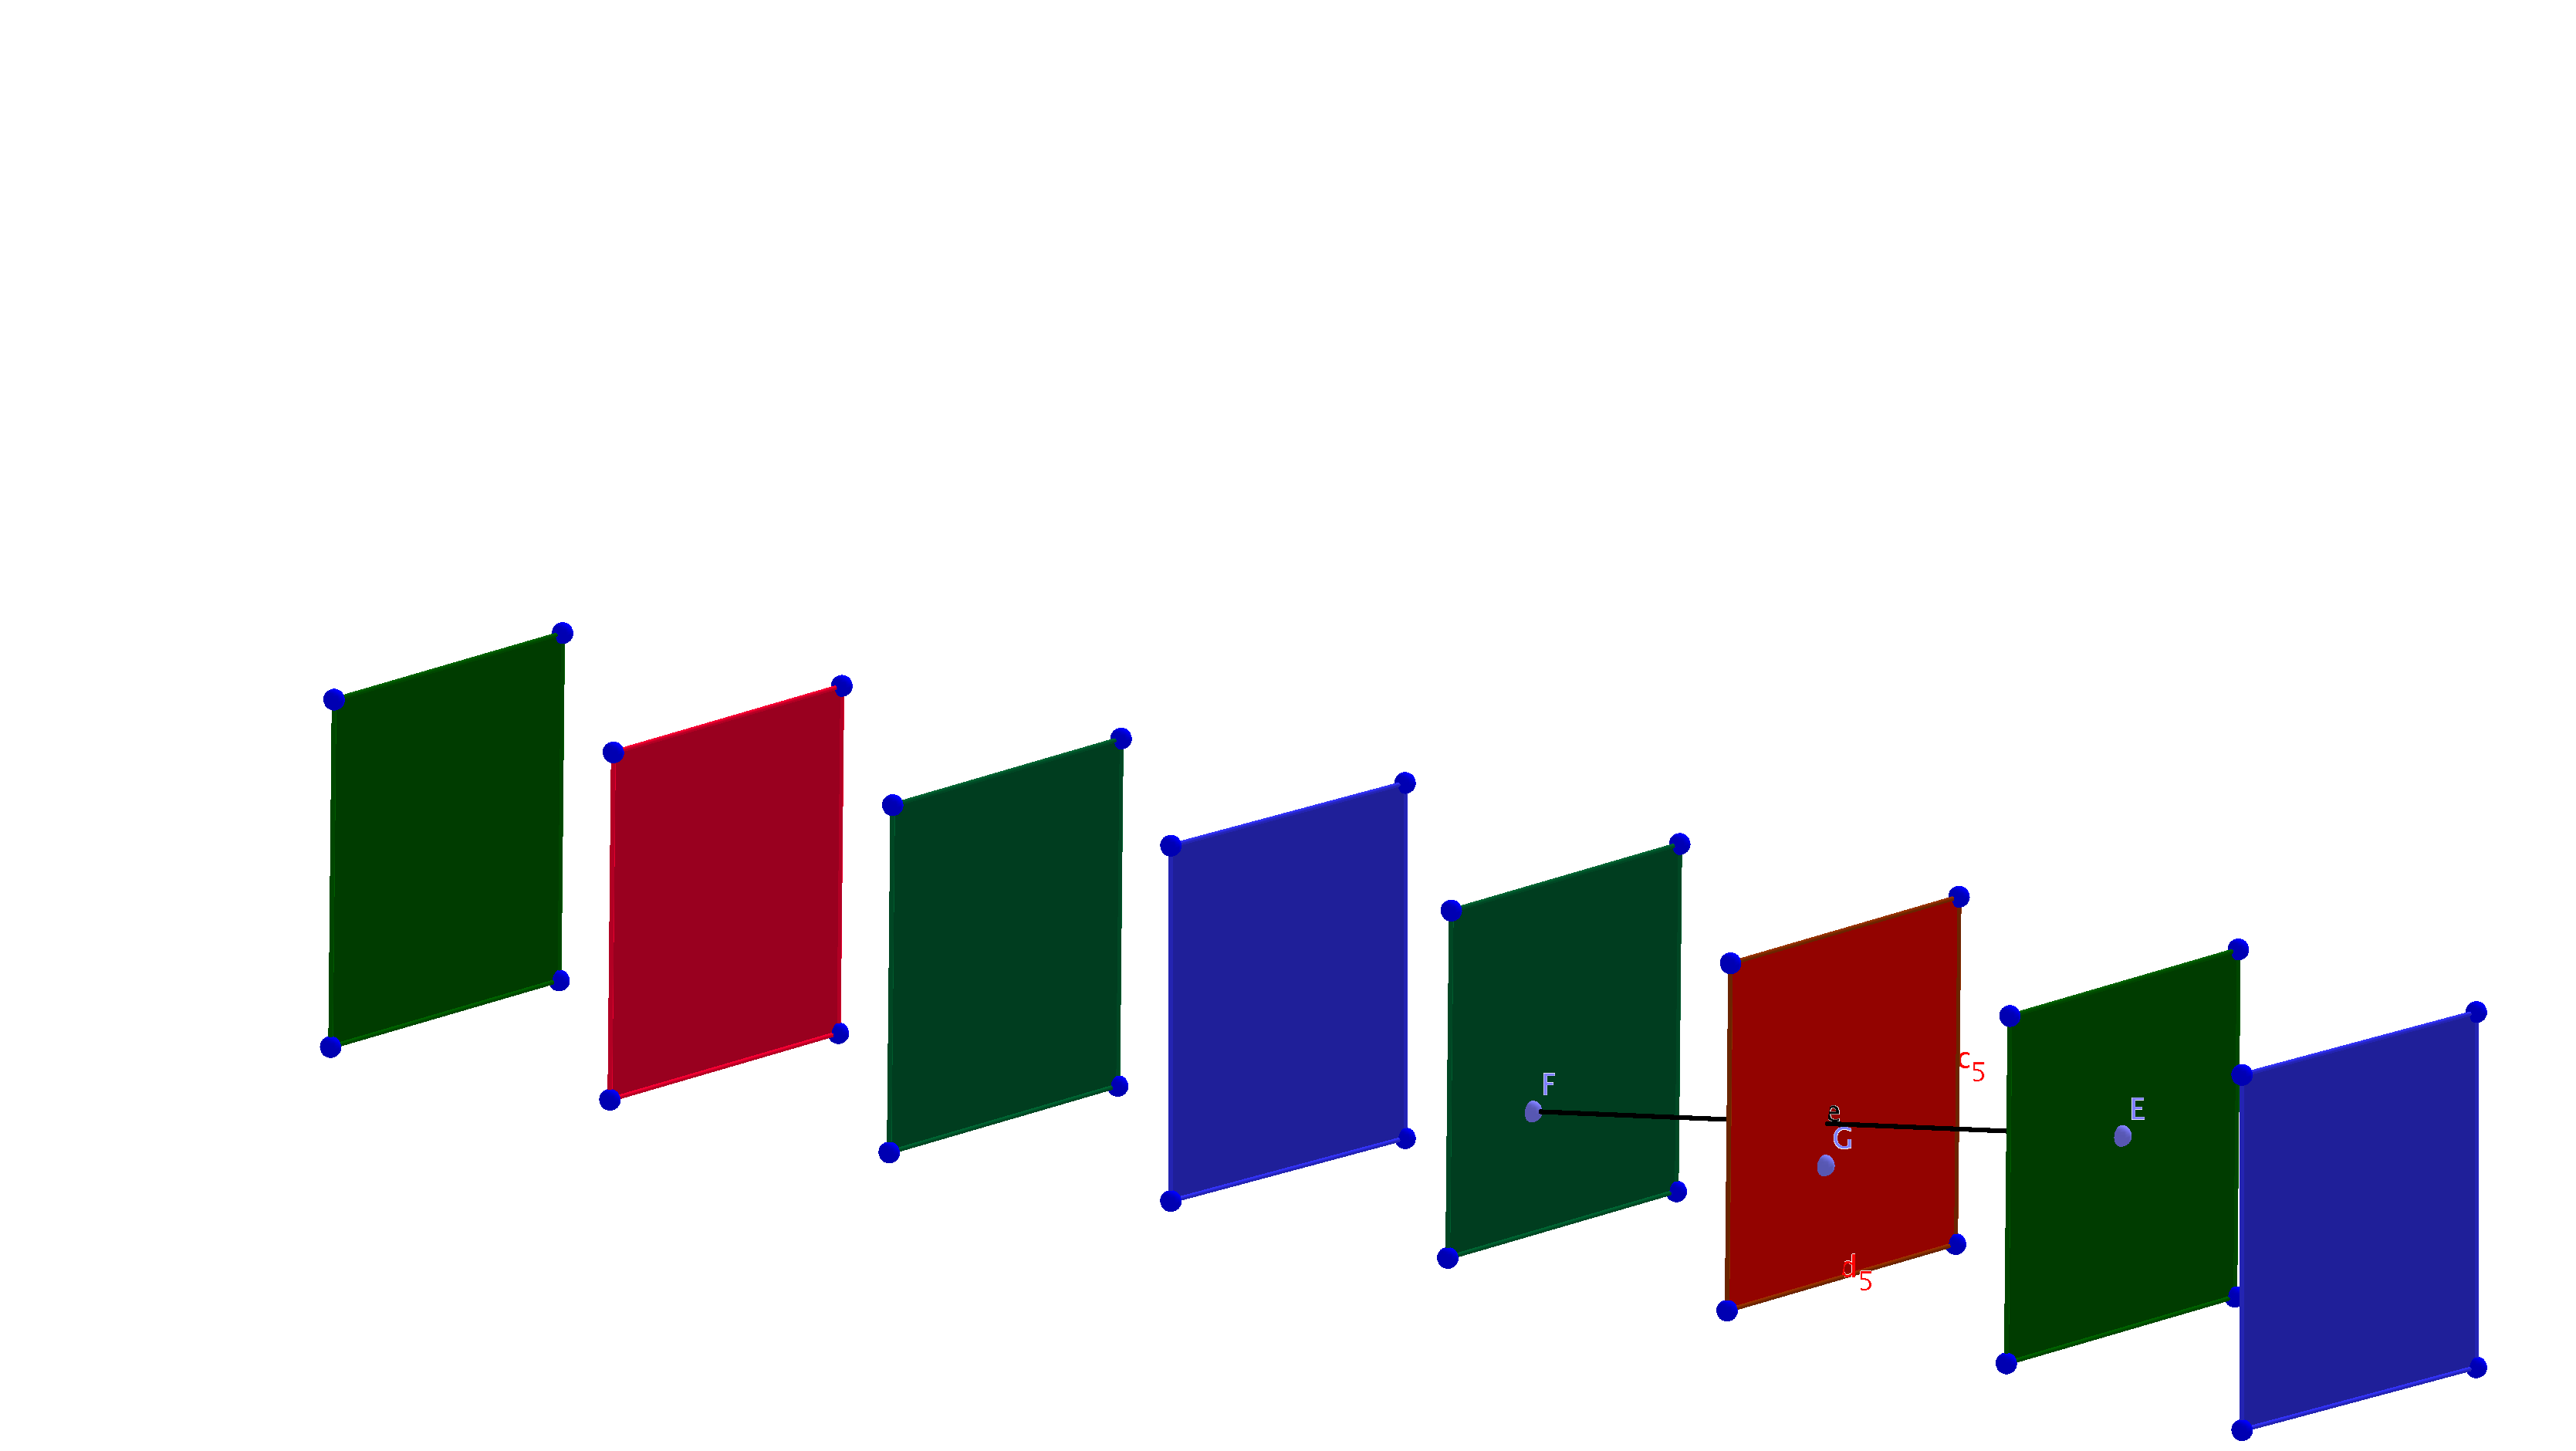
\includegraphics[width=1.0\linewidth]{figures/tripletDoubletFormed.png}
\caption{Doublet which has passed the DoubletDistCut used to look for a triplet. The green planes are used to create the doublets. The red plane with the green planes are used to create the triplets on each arm. The blue planes are DUTs. The blue points are hits.}
\label{fig:TripForm}
\end{figure}

\begin{figure}[H]
\centering
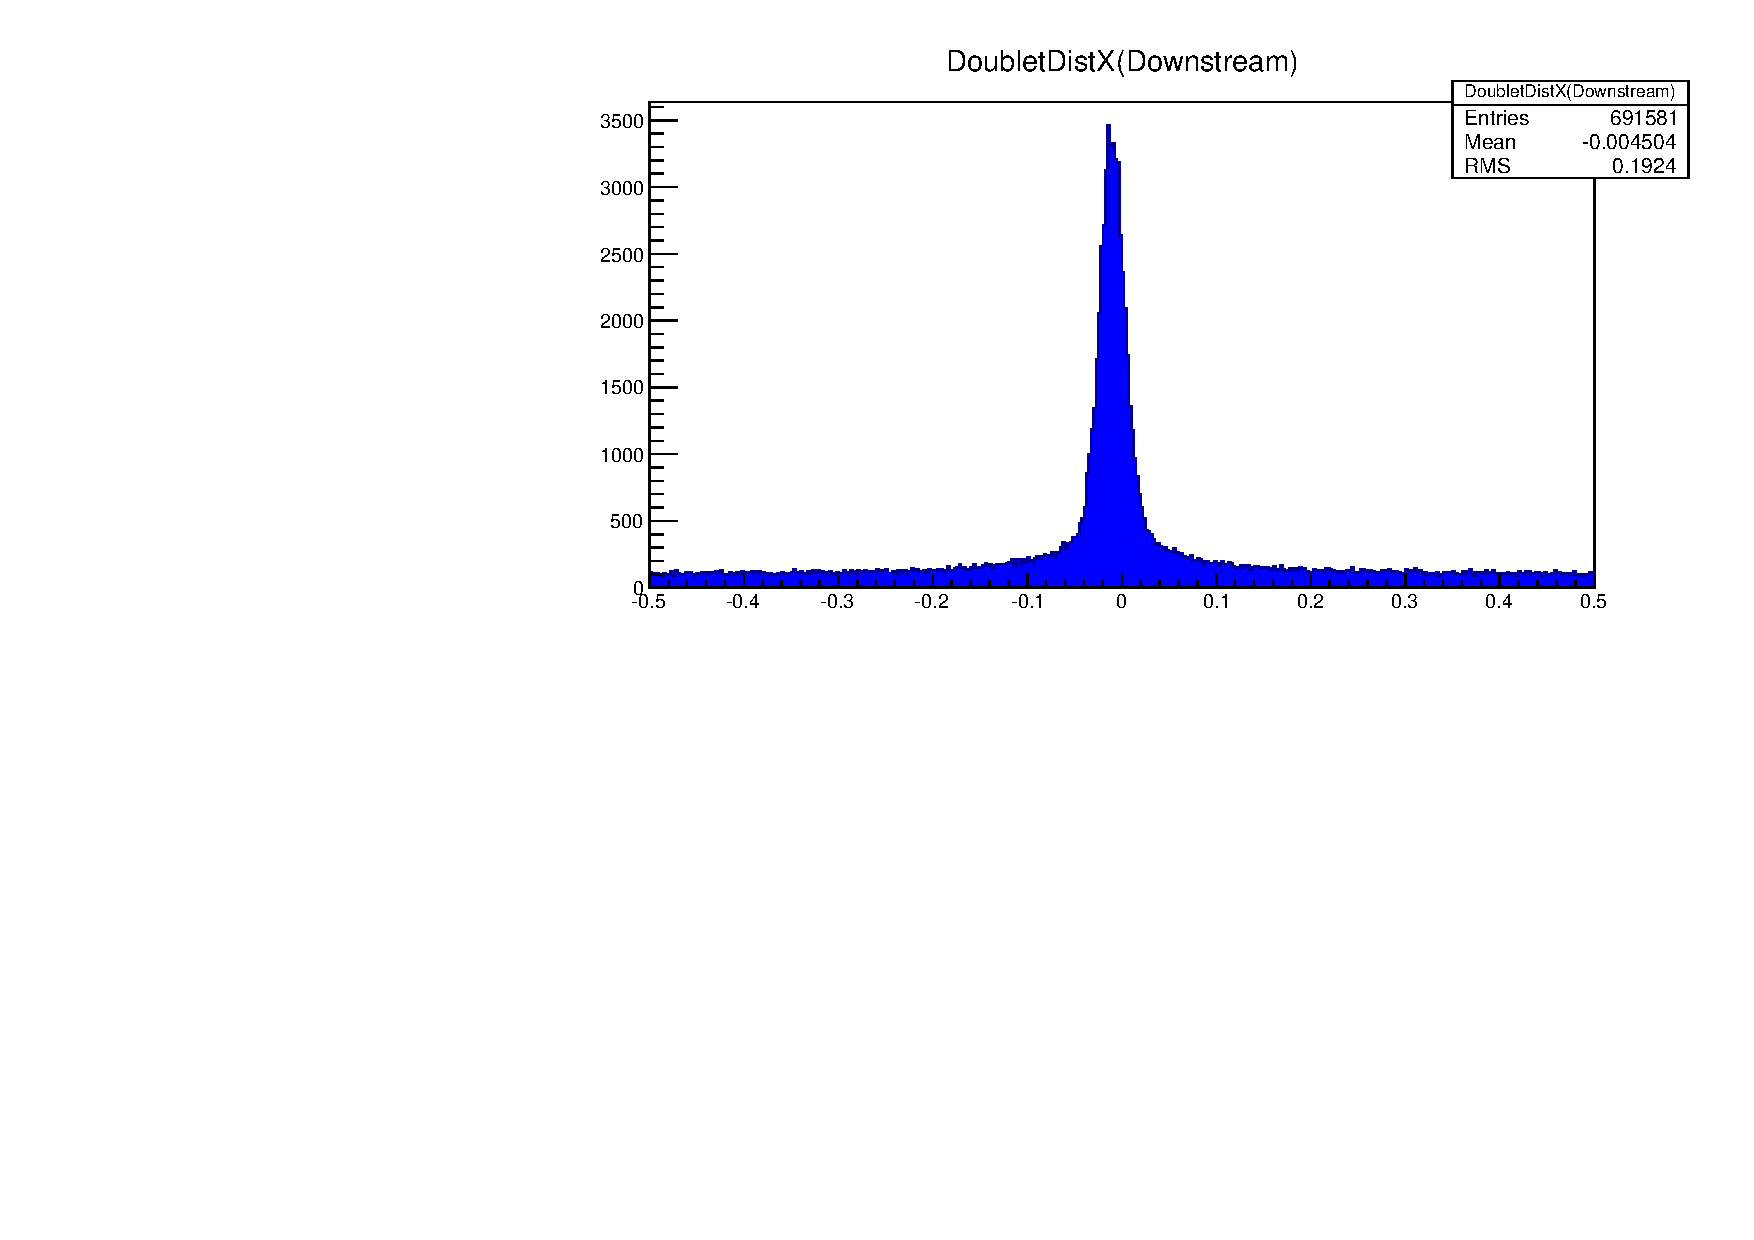
\includegraphics[width=1.0\linewidth]{figures/DoubletDistX-442-preOnly.pdf}
\caption{Doublet distance for down stream arm for DESY testbeam data taken at 4 GeV. This can be used to find the correct cuts for any setup.}
\label{fig:DoubDis}
\end{figure}

\item[DoubletCenDistCut]  The XY plane distance cut on the central planes (Red in figure \ref{fig:TripForm}) and prediction from doublet to create triplet . 

\begin{figure}[H]
\centering
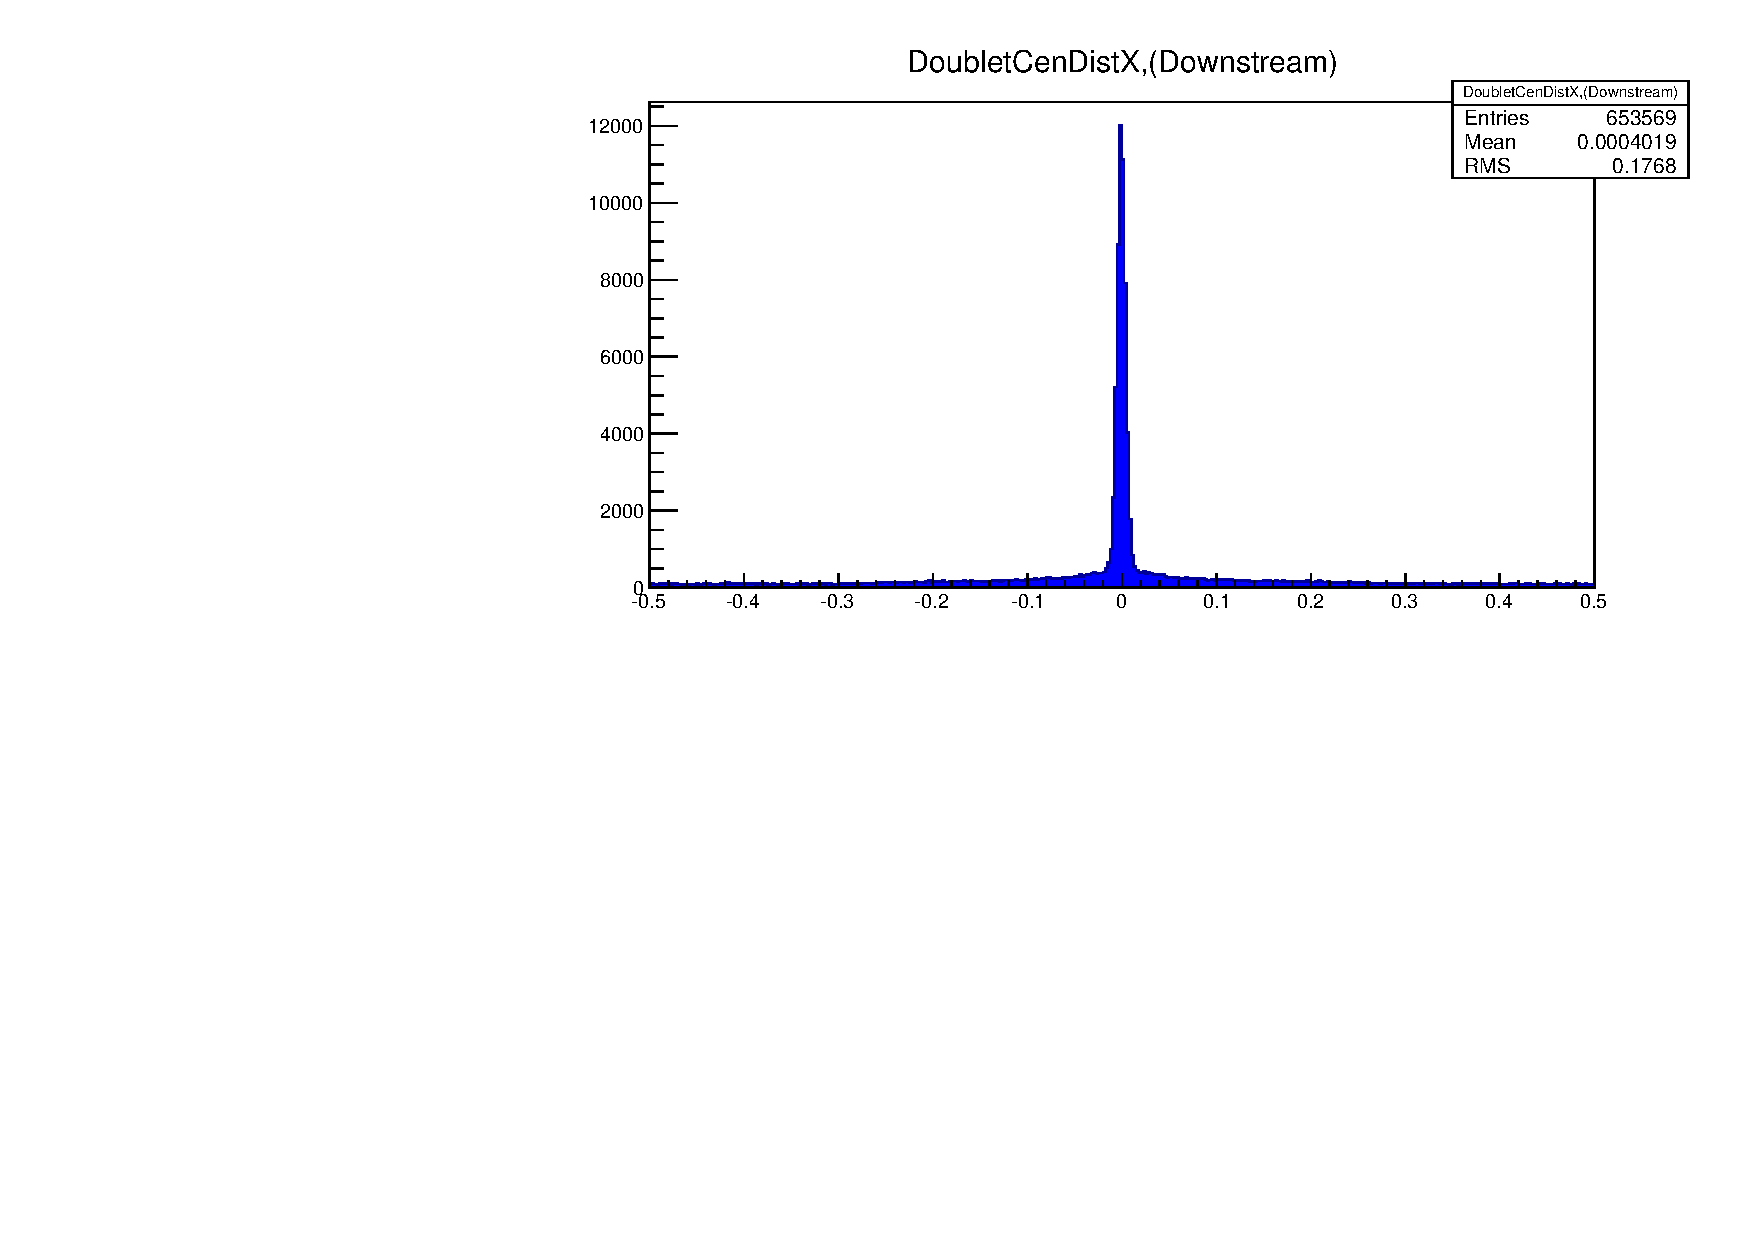
\includegraphics[width=1.0\linewidth]{figures/DoubletCenDist-442.pdf}
\caption{Doublet distance to central hit for down stream arm.}
\label{fig:DoubCen}
\end{figure}

\item[TripletConnectDistCut]  The triplets formed which pass the cuts are associated together using each triplet extrapolated to the centre of both triplets. With each triplet's position defined as the centre of of the doublet. This can be seen in figure \ref{fig:TripCon} were the triplets are extrapolated to a central point near the central DUT (DUTs in blue).

\begin{figure}[H]
\centering
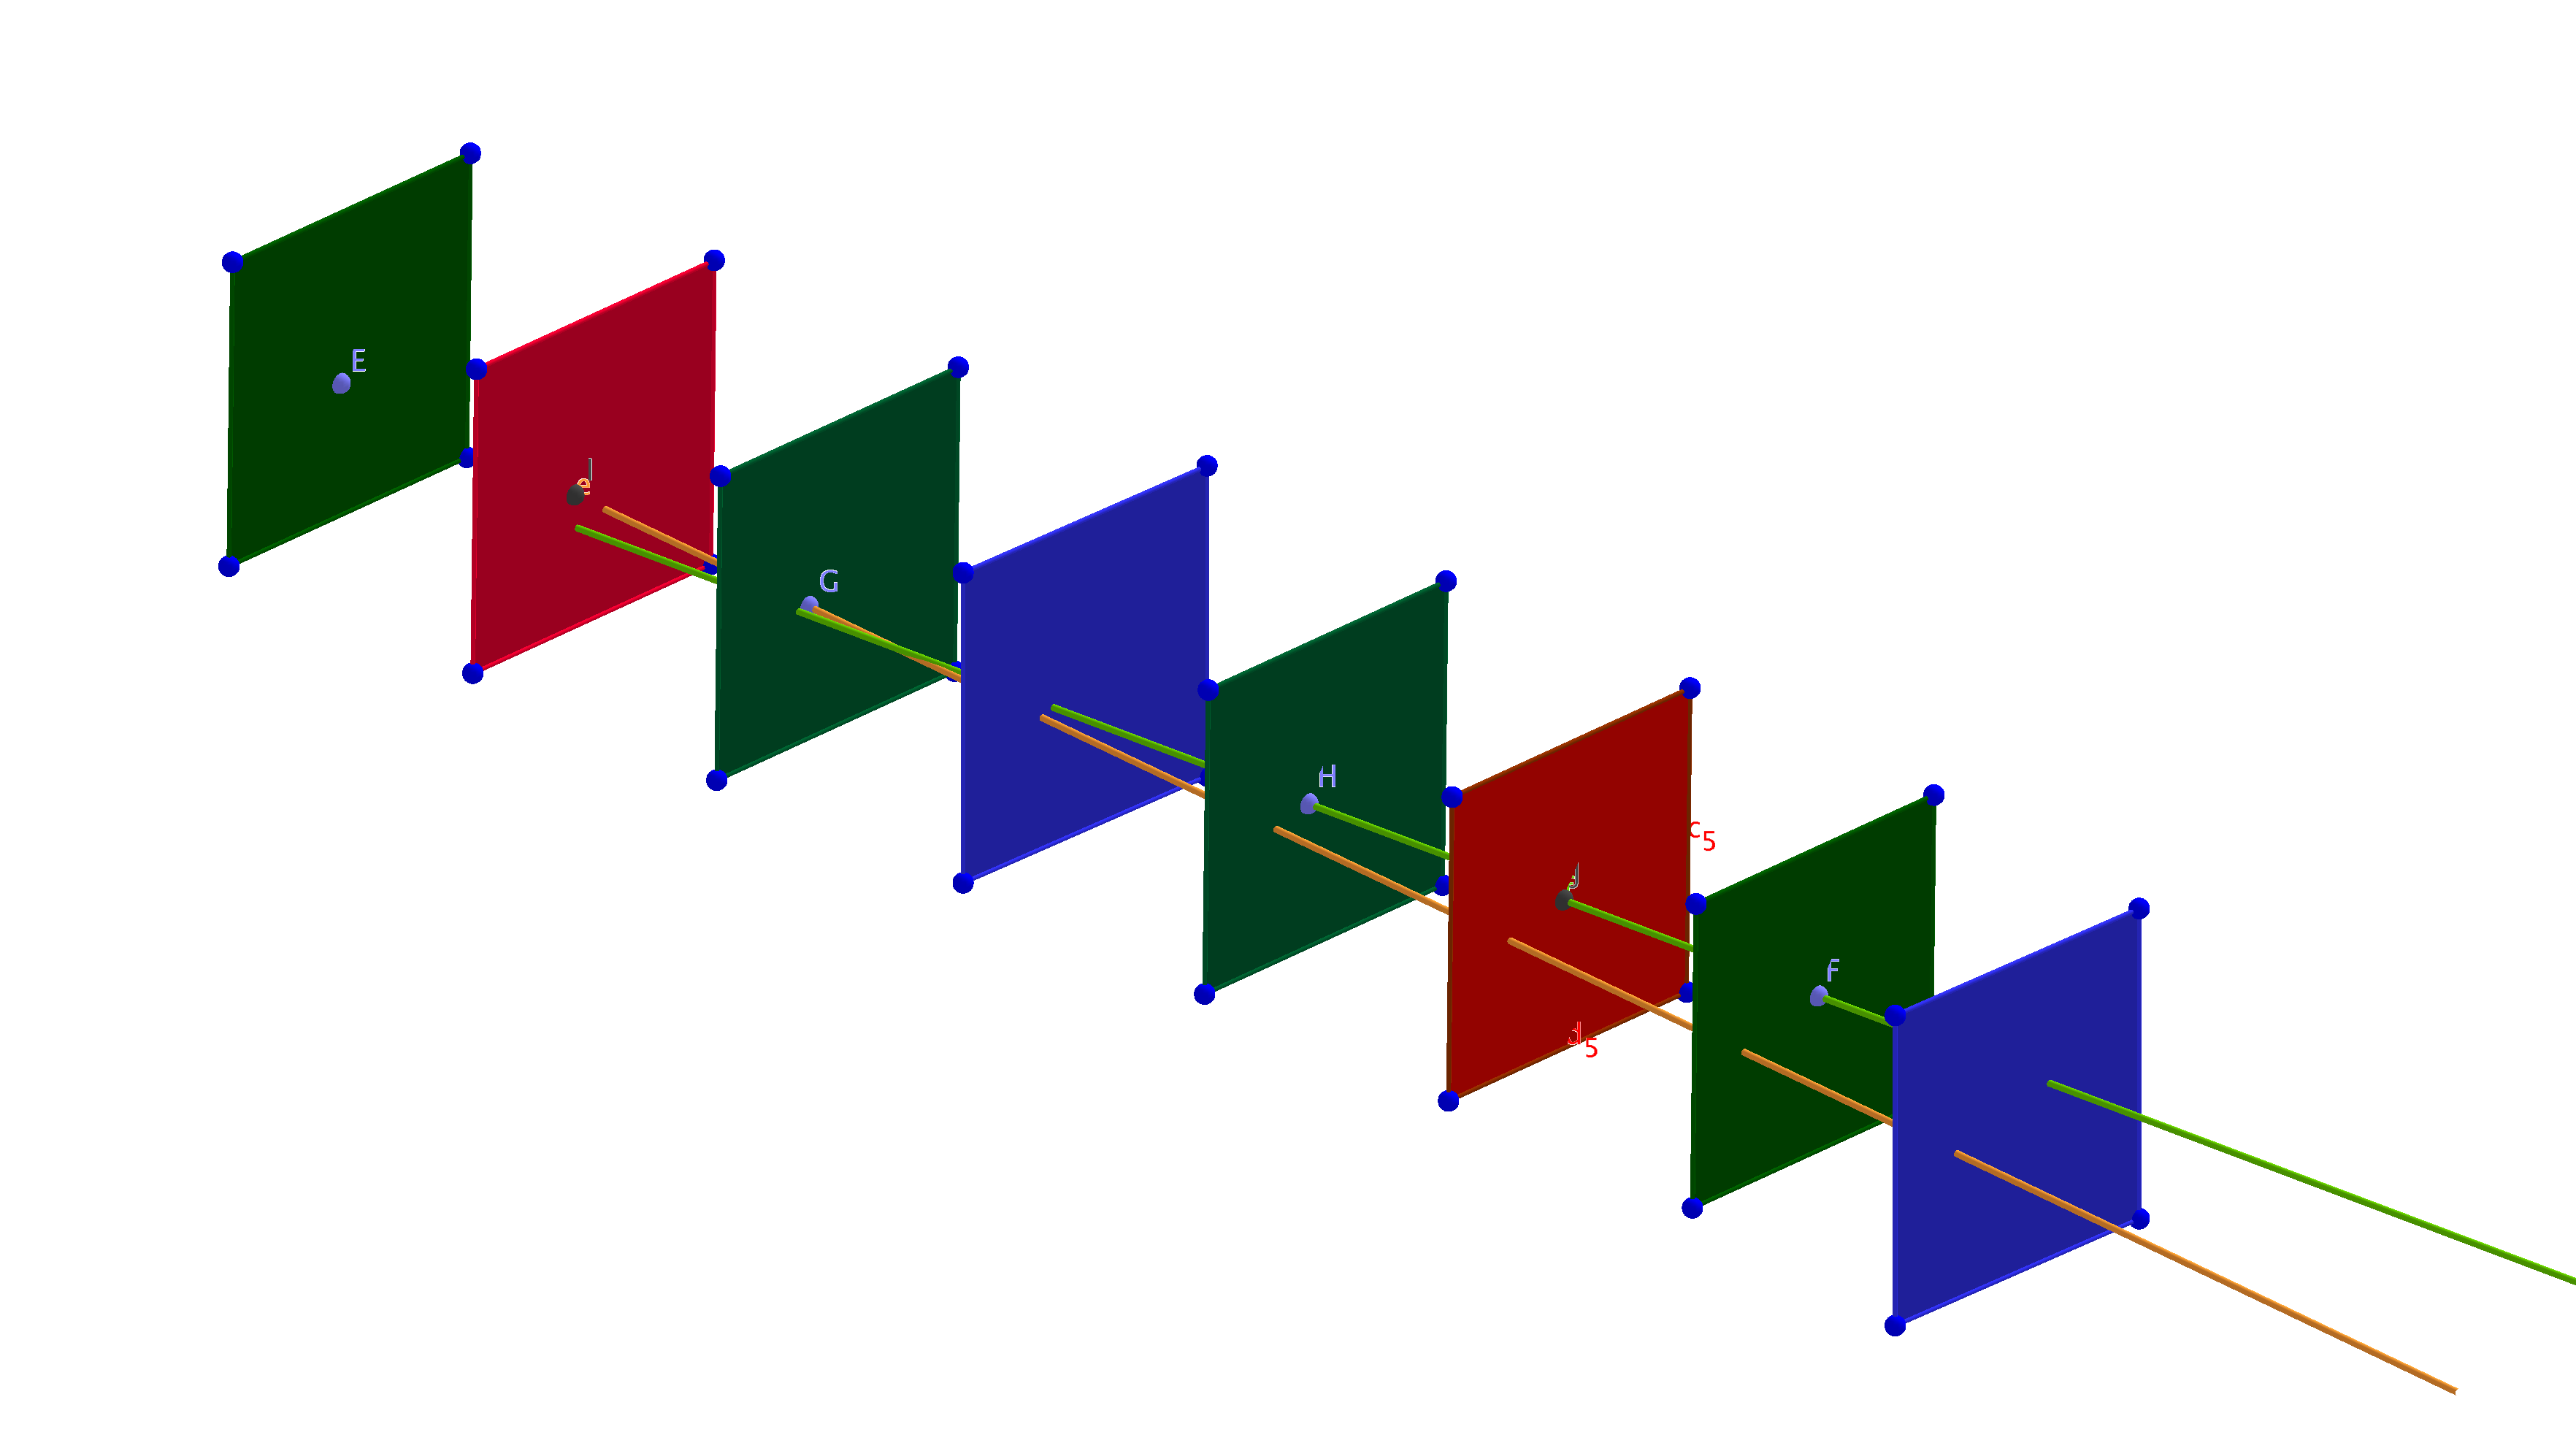
\includegraphics[width=1.0\linewidth]{figures/tripletsconnect.png}
\caption{A central point is used between both arms to compare both triplets' prediction. Each triplet is formed from the green and red planes of each arm. }
\label{fig:TripCon}
\end{figure}

\begin{figure}[H]
\centering
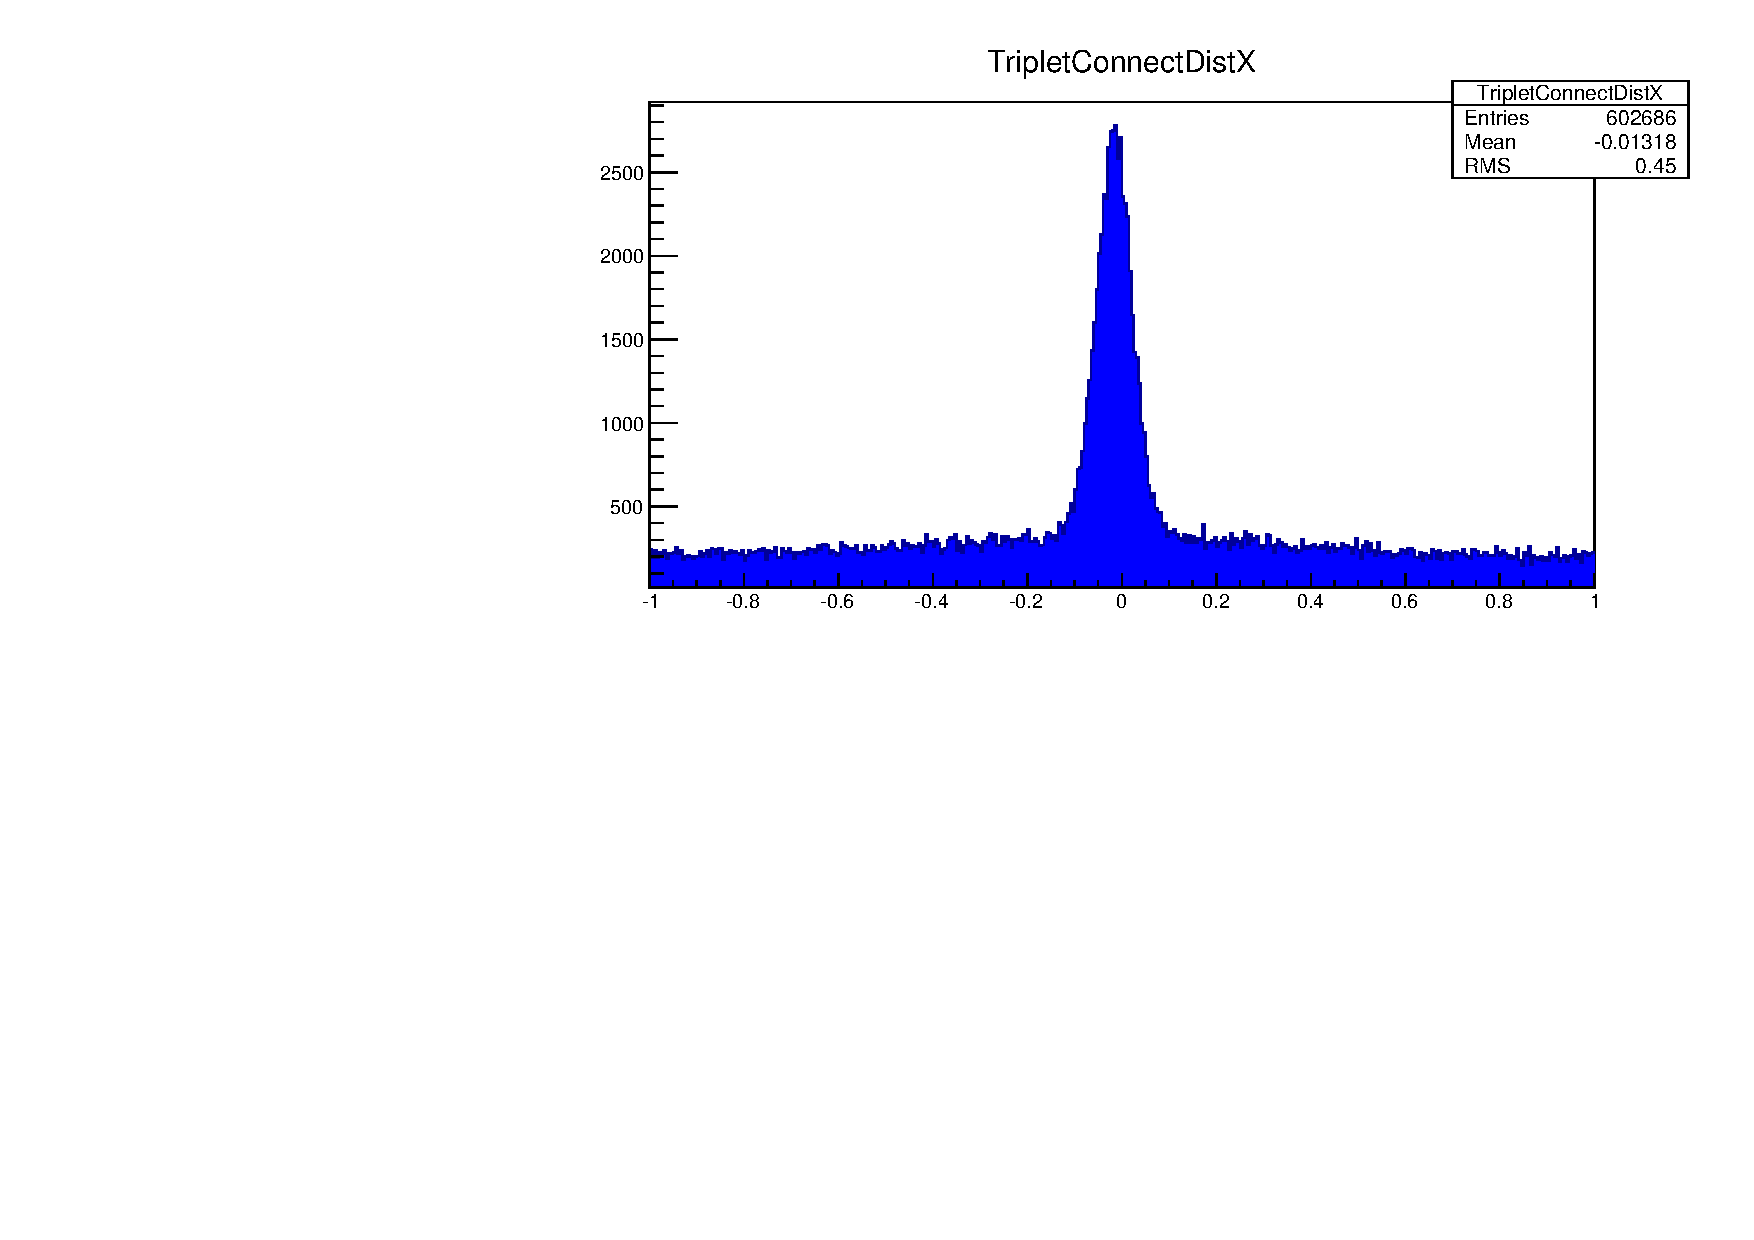
\includegraphics[width=1.0\linewidth]{figures/TripletConnectDistX-442.pdf}
\caption{The distance between the two triplet predictions at some central point.}
\label{fig:TripCen}
\end{figure}

\item[TripletSlopeCut] Figure \ref{fig:TripCon} shows that the prediction of both triplets can be accurate but the slope wrong. Therefore a slope cut between the two triplets must be applied. Testbeam setups in most cases only have a small beam divergence so this does not have to be precise.
\newline
\newline 
beam divergence = approx 1/0.5 mRad (DESY/SLAC)
\newline
\newline
The final track produced before the addition of DUT hits must come from a unique matching of triplets. If a triplet on one arm is matched with two triplets on the other then the triplet with two matches is removed.

\item[DUTWindow] After the triplets are associated together then the DUT hits are attached to this track if the hit is within some minimum distance. 
\begin{figure}[H]
\centering
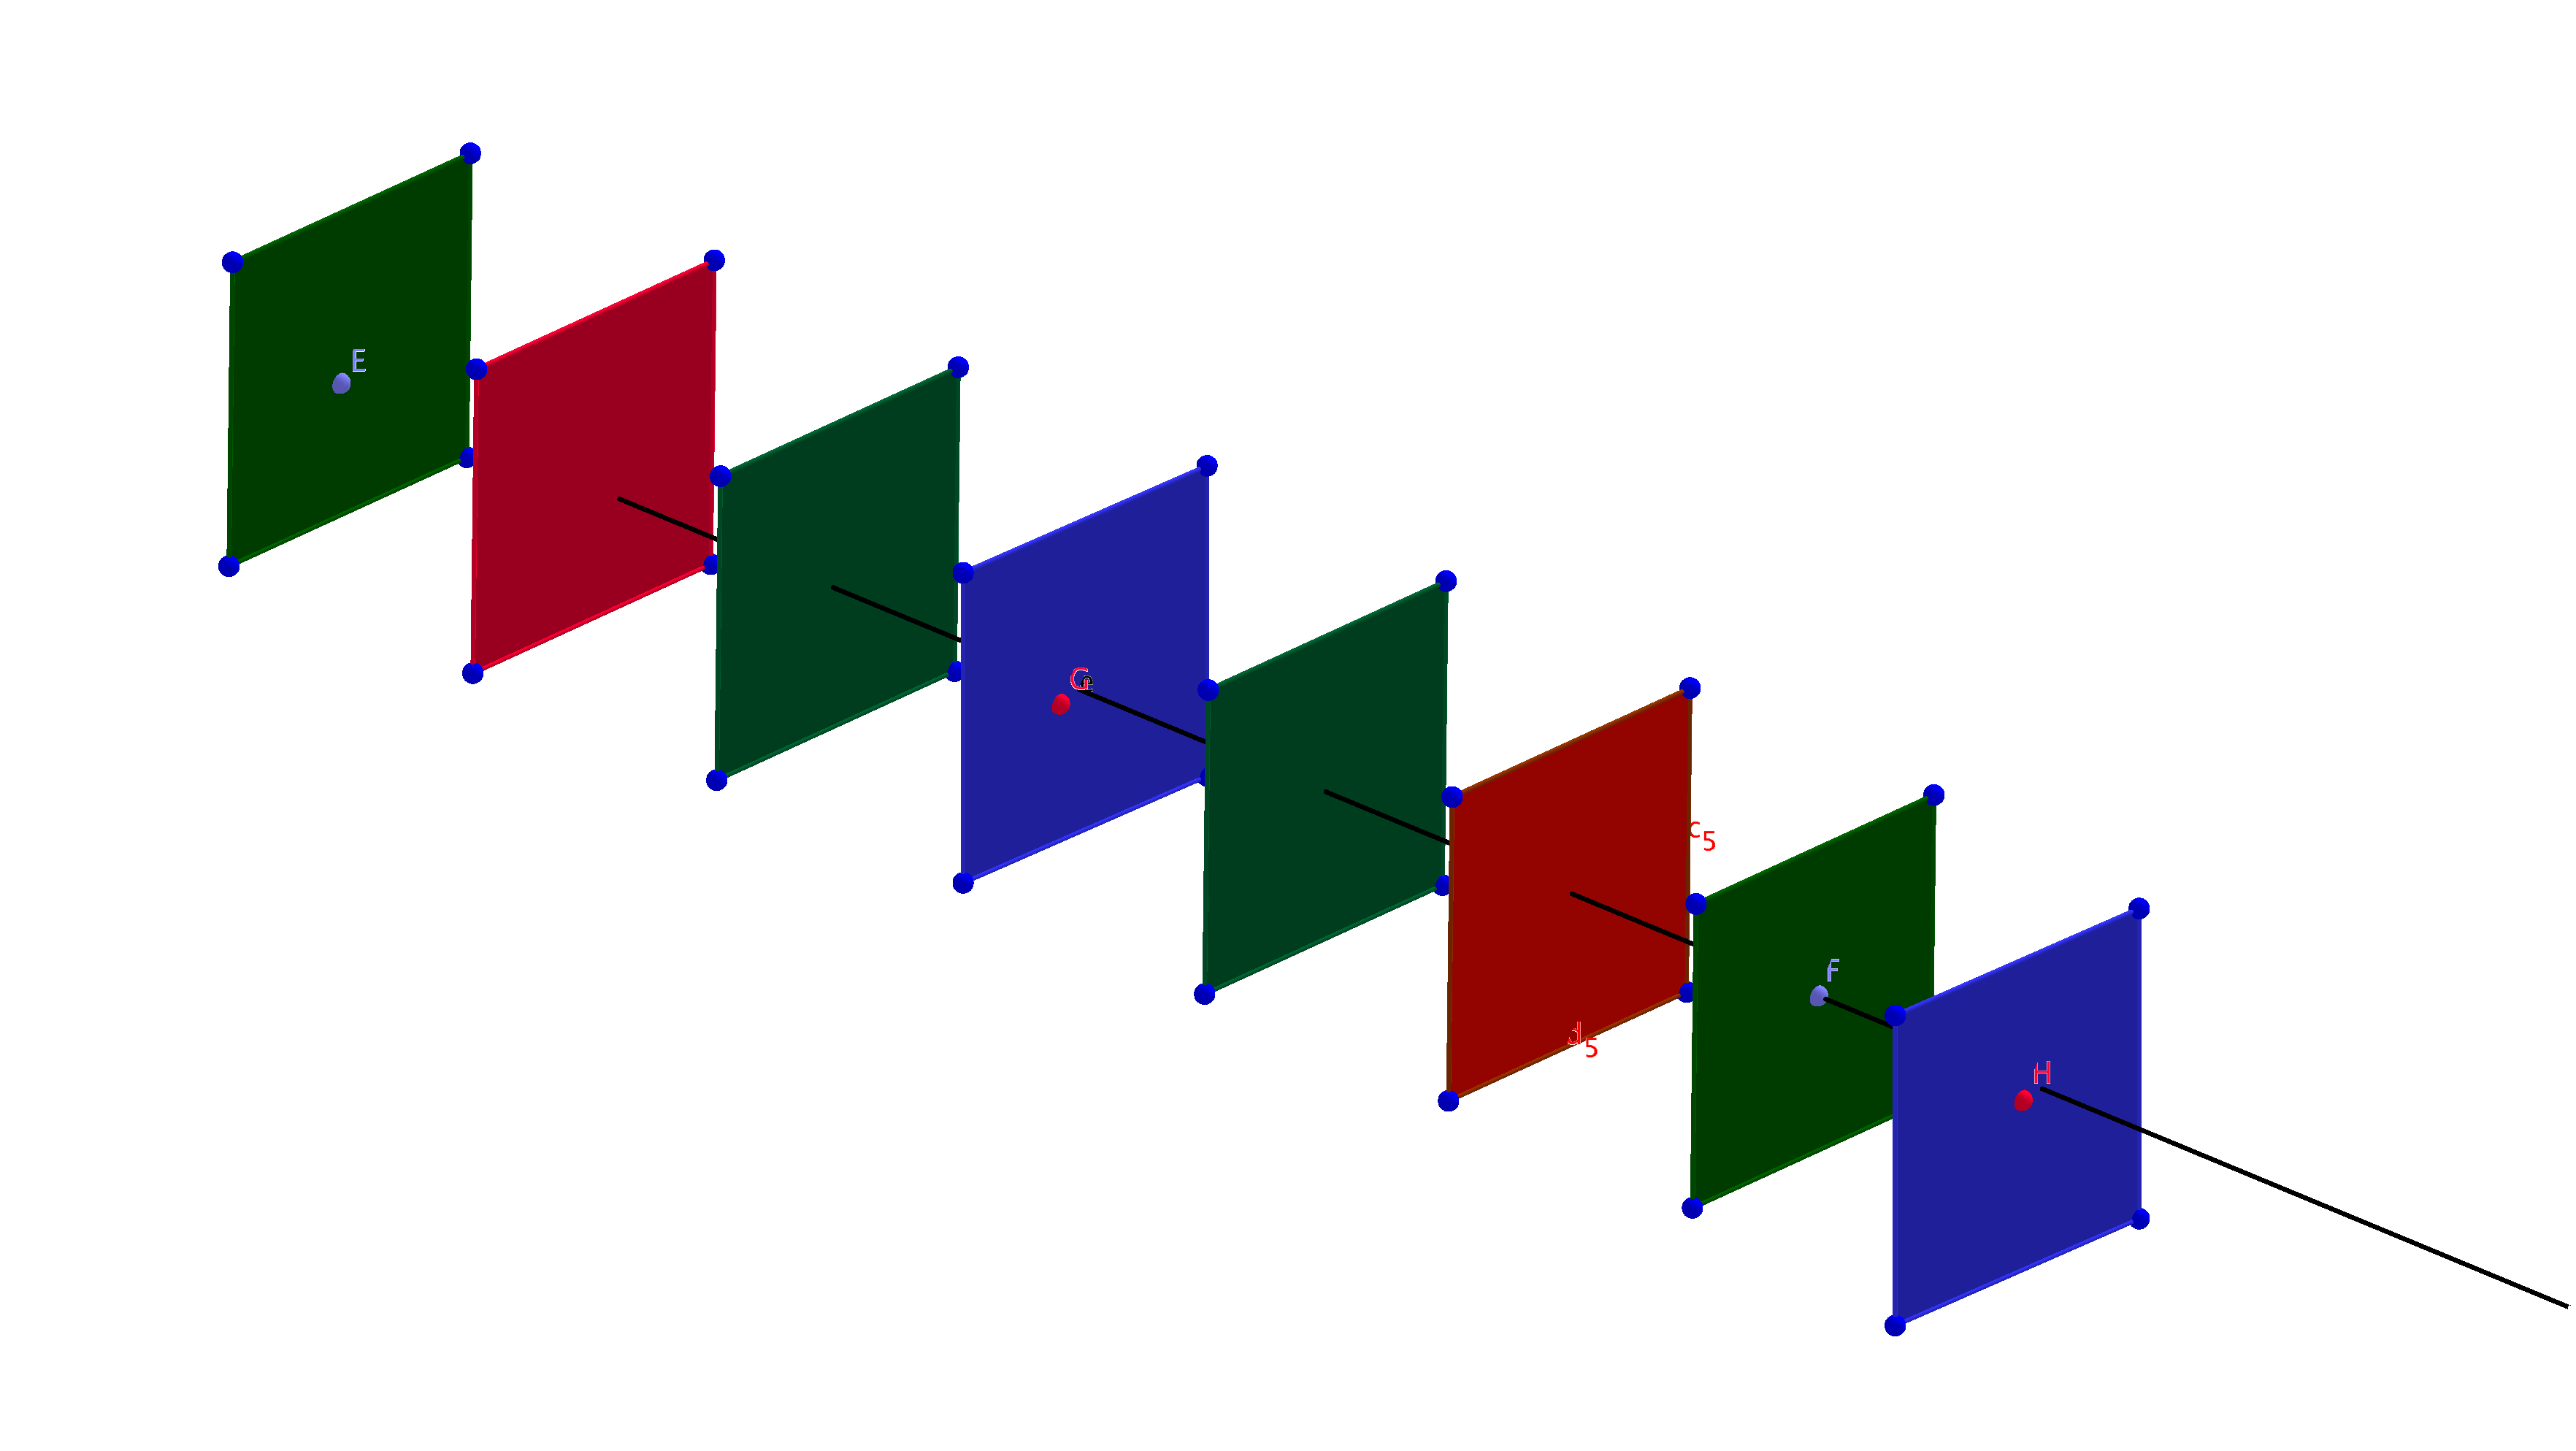
\includegraphics[width=1.0\linewidth]{figures/DUThitsPat.png}
\caption{The red dots on the blue DUT planes are hits. If the track produced by the mimosas is close to these hits then attach the hits to the track.}
\label{fig:DoubDis}
\end{figure}


\end{description}

Unique matching between a single DUT hit and a track must be found. If a track or hit is associated twice then the hit/track is removed from fitting with a DUT hit on that plane. All tracks produced by the mimosas are returned regardless of there being a DUT hit attached.

The hits collected which have been identified are assumed to come from a single track. How this track is described or parameterised depends on how accurate you want to be. Note parameterising is just the same as fitting, however to use the GBL algorithm you need an initial "guess". This initial guess must include positions, incidences, kink angles and curvature. The kink angles are fitted as parameters within GBL in contrast to many fitters which includes this as additional non diagonal variance in the propagated error matrix. In all examples this is not required and a single iteration of the GBL fitter with the basic internal parameterisation will suffice.




